% Reproduction of Barrenechea, John & Knobloch, SINUM 54 (2016), Section 8, with galerkit.
% Tables and figures are generated by examples/convection_diffusion/2d/afc_bjk16/make_report.py.
\documentclass[11pt]{article}

\usepackage[utf8]{inputenc}
\usepackage[T1]{fontenc}
\usepackage{lmodern}
\usepackage[margin=2.5cm]{geometry}
\usepackage{amsmath,amssymb,amsthm,mathtools}
\usepackage{enumitem}
\usepackage{booktabs}
\usepackage{xcolor}
\usepackage{graphicx}
\usepackage{url}
\usepackage[section]{placeins}
\usepackage[colorlinks=true,linkcolor=blue!60!black,citecolor=blue!60!black,urlcolor=blue!60!black]{hyperref}

\newcommand{\mism}[1]{\textcolor{orange!85!black}{#1}}
\newcommand{\eps}{\varepsilon}
\newcommand{\bb}{\boldsymbol{b}}
\newcommand{\R}{\mathbb{R}}

\title{Algebraic flux correction for convection--diffusion--reaction:\\
a reproduction of the numerical results of Barrenechea, John \& Knobloch (SINUM 2016)}
\author{galerkit}
\date{October 2026}

\begin{document}
\maketitle

\begin{abstract}
We recompute all numerical results of Section~8 of G.\,R.~Barrenechea, V.~John and P.~Knobloch, \emph{Analysis of
algebraic flux correction schemes}, SIAM J.\ Numer.\ Anal.\ 54 (2016) 2427--2451~\cite{BJK16}: Example~20 with
$\eps=10^{-8}$ and $\eps=10$ on five grids, Tables~1--11. Of the 252 error values computed (levels~3--8,
up to $1.05\cdot10^{6}$ unknowns), 245 agree with the paper in all four printed digits; the remaining seven differ by
at most $0.08\,\%$, all on levels~7--8 and of the size explained by the paper's looser stopping tolerance. The
reproduction settles three points the paper leaves implicit: Table~1 is computed on grid~5 (as its caption says,
not on grid~1 as the text says), the mean in Table~7 is taken over all edges, and the error norm $\|e_h\|_h$ uses
$C_a=1$ with the stabilisation term evaluated at $i_hu-u_h$. The unstructured grid~3, not given in the paper, was
recovered exactly from the vector drawing of its Figure~1. The fixed-point iteration with Anderson acceleration used
in the paper is, on the non-Delaunay and unstructured grids at $\eps=10^{-8}$, more than ten times faster than a
semismooth Newton method; on grid~3 at level~7 both stagnate at a residual of $1.3\cdot10^{-8}$.
\end{abstract}

\tableofcontents

%=====================================================================================================
\section{Scope and summary}
%=====================================================================================================

The paper~\cite{BJK16} proves, for algebraic flux correction (AFC) schemes with symmetric limiters, existence of
solutions, a local discrete maximum principle for Kuzmin's limiter, and an a~priori error estimate for the
convection--diffusion--reaction equation (Corollary~17). Its Section~8 tests the estimate on one smooth example with
eleven tables. We recompute every table with the finite element code \texttt{galerkit}; Table~S
lists the agreement table by table and the cost of the finest solve, Figure~\ref{fig:conv} shows the two quantities
the theory is about, and Section~\ref{sec:results} gives every table.

% generated by make_report.py; do not edit
\begin{table}[!htbp]
\renewcommand{\thetable}{S}
\centering\small\setlength{\tabcolsep}{4pt}
\caption{Agreement with the paper per table: entries computed, entries differing in the printed digits, largest relative deviation from the printed values (the printing rounds by up to $5\cdot10^{-4}$), and the nonlinear solve on the finest level (solver and iterations, final Euclidean residual, wall time in minutes on one core).}\label{tab:bjk16-summary}
\begin{tabular}{rrrcrrrlrr}
\toprule
Table & $\varepsilon$ & grid & levels & entries & differ & max dev. & finest: solver, it. & residual & min\\
\midrule
1 & $10^{-8}$ & 5 & 3--8 & 24 & 0 & 3.7e-04 & Newton 1 & 1e-16 & 5 \\
2 & $10^{-8}$ & 1 & 3--8 & 24 & 4 & 7.9e-04 & Anderson 3688 & 1e-10 & 95 \\
3 & $10^{-8}$ & 2 & 3--7 & 20 & 0 & 3.7e-04 & Newton 42 & 2e-16 & 3 \\
4 & $10^{-8}$ & 3 & 3--7 & 20 & 1 & 2.9e-04 & Anderson 3400 & 1e-08 & 13 \\
5 & $10^{-8}$ & 4 & 3--8 & 24 & 1 & 2.5e-04 & Anderson 7066 & 1e-10 & 173 \\
6 & $10^{-8}$ & 5 & 3--8 & 24 & 1 & 3.0e-04 & Anderson 6833 & 1e-10 & 168 \\
8 & $10$ & 1 & 3--7 & 20 & 0 & 4.1e-04 & Newton 2 & 6e-13 & 1 \\
9 & $10$ & 4 & 3--8 & 24 & 0 & 3.0e-04 & Newton 1 & 2e-11 & 5 \\
10 & $10$ & 5 & 3--8 & 24 & 0 & 3.7e-04 & Newton 4 & 1e-12 & 8 \\
11 & $10$ & 5 & 3--8 & 24 & 0 & 4.2e-04 & Newton 2 & 1e-12 & 10 \\
\bottomrule
\end{tabular}
\end{table}


The main findings are:
\begin{enumerate}[leftmargin=*]
\item \textbf{The results are reproduced.} Every printed digit agrees except seven entries, all on the two finest
  levels: four in Table~2, one each in Tables~4, 5 and~6 (Section~\ref{sec:dev}).
\item \textbf{Three implicit choices of the paper are identified} (Section~\ref{sec:clar}): the grid of Table~1,
  the averaging set of Table~7, and the precise form of $\|e_h\|_h$.
\item \textbf{Solver.} Anderson-accelerated fixed point iteration, as in the paper, is the method of choice for
  $\eps=10^{-8}$ on grids~3--5; semismooth Newton is faster everywhere else (Section~\ref{sec:solvers}).
\item \textbf{What the data say about the theory} (Section~\ref{sec:theory}): the $O(h^{1/2})$ estimate of
  Corollary~17 is attained for solution-independent weights and is pessimistic for Kuzmin's limiter on grid~1;
  in the diffusion-dominated regime the convergence of $d_h(u_h;i_hu,i_hu)^{1/2}$ is decided by the mesh angles
  exactly as Remark~18 predicts.
\end{enumerate}

%=====================================================================================================
\section{Problem, scheme and error measures}\label{sec:setup}
%=====================================================================================================

\paragraph{Example 20.} On $\Omega=(0,1)^2$,
\begin{equation}\label{eq:pde}
  -\eps\Delta u+\bb\cdot\nabla u+cu=g\ \ \text{in }\Omega,\qquad u=0\ \ \text{on }\partial\Omega,\qquad
  \bb=(3,2)^T,\ c=1,
\end{equation}
with $g$ such that $u(x,y)=100\,x^2(1-x)^2\,y(1-y)(1-2y)$, for $\eps=10^{-8}$ (convection dominated) and $\eps=10$
(diffusion dominated). Here $\sigma_0=c=1$.

\paragraph{AFC scheme.} Let $A=(a_{ij})_{i,j=1}^N$ be the $P_1$ Galerkin matrix of \eqref{eq:pde} with natural
boundary conditions, the reaction term mass-lumped (row sums), and $x_{M+1},\dots,x_N$ the Dirichlet nodes. With the
artificial diffusion matrix
\begin{equation}\label{eq:d9}
  d_{ij}=d_{ji}=-\max\{a_{ij},0,a_{ji}\}\quad(i\neq j),\qquad d_{ii}=-\textstyle\sum_{j\neq i}d_{ij},
\end{equation}
and the fluxes $f_{ij}=d_{ij}(u_j-u_i)$, the scheme reads~\cite[(11)]{BJK16}
\begin{equation}\label{eq:afc}
  \sum_{j=1}^N a_{ij}u_j+\sum_{j\neq i}\bigl(1-\alpha_{ij}(u)\bigr)d_{ij}(u_j-u_i)=g_i,\quad i=1,\dots,M,
  \qquad u_i=0,\ i>M .
\end{equation}

\paragraph{Limiter.} Kuzmin's limiter as stated in~\cite[Sect.~4]{BJK16}: for $a_{ji}\le a_{ij}$ (node $i$
``owns'' the edge),
\[
  P_i^\pm=\sum_{j:\,a_{ji}\le a_{ij}}f_{ij}^\pm,\quad Q_i^\pm=-\sum_{j}f_{ij}^\mp,\quad
  R_i^\pm=\min\{1,Q_i^\pm/P_i^\pm\},\quad
  \alpha_{ij}=\alpha_{ji}=\begin{cases}R_i^+,&f_{ij}>0,\\1,&f_{ij}=0,\\R_i^-,&f_{ij}<0,\end{cases}
\]
with $R_i^\pm=1$ when $P_i^\pm=0$ and at Dirichlet nodes, so that $\alpha_{ij}=1$ on edges owned by a Dirichlet node.

\paragraph{Variants.} Table~1 uses the solution-independent weights $\alpha_{ij}=0.5$ (with $\alpha_{ij}=1$ on edges
owned by a Dirichlet node, as in the paper); the problem is then linear. Table~11 replaces \eqref{eq:d9} by the
convection matrix alone,
\begin{equation}\label{eq:d54}
  d_{ij}=-\max\{(\bb\cdot\nabla\varphi_j,\varphi_i),\,0,\,(\bb\cdot\nabla\varphi_i,\varphi_j)\}\qquad(i\neq j),
\end{equation}
which is~\cite[(54)]{BJK16}.

\paragraph{Error measures.} With $e_h=u-u_h$ and $i_h$ the nodal interpolant, the tables report
$\|e_h\|_{0}$, $|e_h|_{1}$,
\[
  d_h(u_h)^{1/2}:=d_h(u_h;i_hu,i_hu)^{1/2},\qquad
  d_h(w;v,v)=\sum_{i<j}\bigl(1-\alpha_{ij}(w)\bigr)|d_{ij}|\,(v_i-v_j)^2,
\]
and
\begin{equation}\label{eq:normh}
  \|e_h\|_h^2=C_a\bigl(\eps|e_h|_{1}^2+\sigma_0\|e_h\|_{0}^2\bigr)+d_h(u_h;i_hu-u_h,i_hu-u_h),\qquad C_a=1 .
\end{equation}
The paper defines $\|\cdot\|_h$ on the discrete space with an unspecified constant $C_a$; \eqref{eq:normh} is the
reading that reproduces all its values (e.g.\ $\eps=10$, grid~1, level~3: $\sqrt{10}\,|e_h|_1=0.5556$ against
$\|e_h\|_h=0.5557$ printed).

%=====================================================================================================
\section{Grids}\label{sec:grids}
%=====================================================================================================

\begin{figure}[!htbp]
\centering
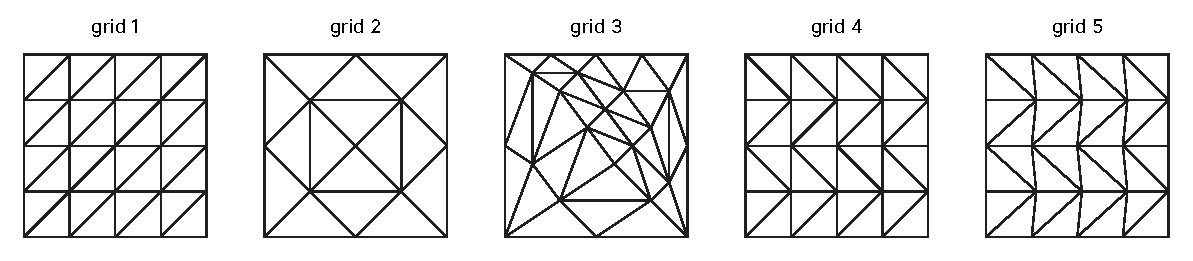
\includegraphics[width=\textwidth]{figures/bjk16_grids.pdf}
\caption{Grids 1--5 on level 0 as built by \texttt{run\_bjk16.py}; compare~\cite[Fig.~1]{BJK16}.}
\label{fig:grids}
\end{figure}

Figure~\ref{fig:grids} shows the five grids on level~0.
\begin{itemize}[leftmargin=*]
\item \textbf{Grid 1}: $4\times4$ squares, Friedrichs--Keller diagonals ``/''.
\item \textbf{Grid 2}: 13 nodes and 16 triangles: the diamond through the edge midpoints and the square
  $[\frac14,\frac34]^2$ with both diagonals.
\item \textbf{Grid 3}: unstructured, 24 nodes and 36 triangles. The paper gives no coordinates. Its Figure~1 is
  vector graphics (a \texttt{gnuplot} file \texttt{grid\_irregular.eps}); reading the drawing commands from the PDF
  gives the triangle list exactly, and all nodes turn out to be multiples of $1/20$. A random Delaunay grid of
  the same size, tried first, misses the paper's values by about $30\,\%$; the extracted grid reproduces them.
\item \textbf{Grid 4}: grid~1 with ``\textbackslash'' diagonals in the even rows of squares (counted from below).
\item \textbf{Grid 5}: grid~4 with the interior nodes of the even horizontal mesh lines shifted to the right by
  $h/10$, so that $\theta_{ij}>\pi/2$ for every diagonal edge (non-Delaunay).
\end{itemize}
Level $l$ of grids 1, 4, 5 has $4\cdot2^l$ squares per side, $h=2^{-l-2}$; grids~2 and~3 are refined uniformly
(red refinement) $l$ times. Level~8 has $1\,050\,625$ nodes on grids 1, 4, 5.

%=====================================================================================================
\section{Nonlinear solvers}\label{sec:solvers}
%=====================================================================================================

The paper solves \eqref{eq:afc} by a fixed-point iteration with Anderson acceleration~\cite{WN11} and stops when the
Euclidean norm of the residual is below $10^{-9}$. We use two solvers, both stopped at $10^{-10}$.
\begin{itemize}[leftmargin=*]
\item \textbf{Semismooth Newton} with the exact generalised Jacobian of the limiter on its current smooth branch and an
  Armijo line search (default).
\item \textbf{Anderson-accelerated fixed point} (\texttt{fp\_anderson}): the map
  $u\mapsto\tilde u$, $(A+D)\tilde u=g-L\bigl((1-\alpha(u))d-d\bigr)u$, where $L(w)$ is the graph Laplacian with edge
  weights $w$, so that one LU factorisation of $A+D$ serves all iterations; Anderson mixing of depth~10 in the form
  of~\cite[Sect.~3]{WN11}; if the best residual has not halved within 200 iterations, the history is cleared and the
  iteration restarts from the best iterate.
\end{itemize}

Both give the same values to all printed digits wherever both converge. Their costs differ sharply:
\begin{itemize}[leftmargin=*]
\item For $\eps=10$ and for $\eps=10^{-8}$ on grids~1 and~2, Newton needs 1--42 iterations on every level.
\item For $\eps=10^{-8}$ on grids~3--5 the number of Newton steps grows quickly (grid~4: 22, 34, 233 on levels 4, 5, 6),
  and on grid~4 level~7 Newton had not converged after four hours. Anderson solves grids~4 and~5 on level~7 in
  5122 and 4984 iterations (21 and 20 minutes), and on level~8 in about 7000 iterations (under three hours).
\item On \textbf{grid 3, level 7}, Anderson converges linearly to a residual of $1.4\cdot10^{-8}$ and then stagnates;
  clearing the history does not help, and Newton started from that iterate only takes steps of length
  $10^{-3}$--$10^{-4}$. The stagnation is therefore a property of the nonlinear problem (switching of the limiter at
  near-ties of nodal values) and not of the acceleration. The row of Table~\ref{tab:bjk16-t4} for level~7 is the
  Anderson iterate after 3400 iterations, residual $1.35\cdot10^{-8}$. Its errors agree with the paper in all
  printed digits except $\|e_h\|_h=9.6499\cdot10^{-4}$ against $9.649\cdot10^{-4}$.
\end{itemize}

%=====================================================================================================
\section{Results}\label{sec:results}
%=====================================================================================================

\begin{figure}[!htbp]
\centering
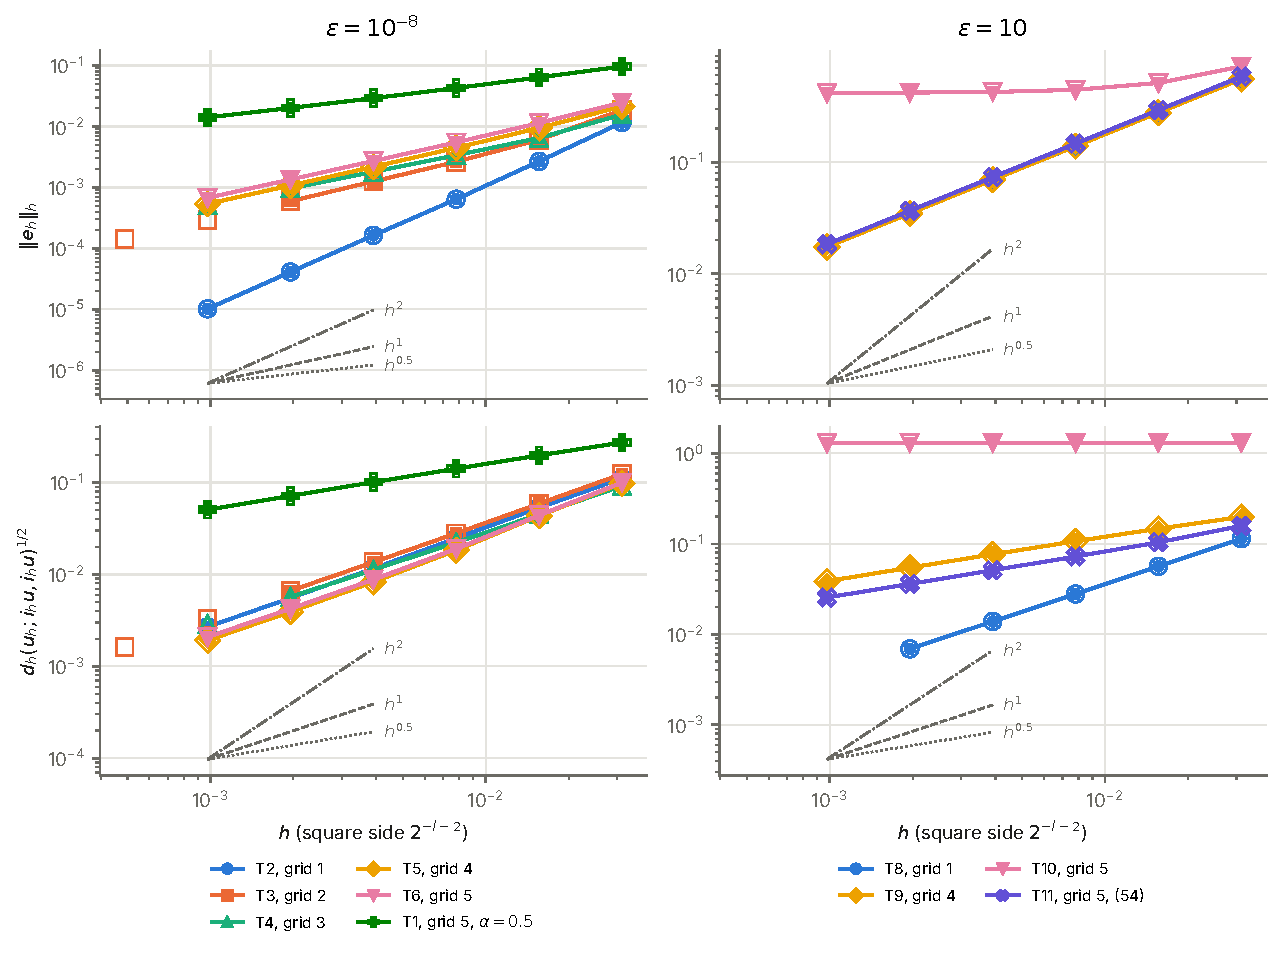
\includegraphics[width=\textwidth]{figures/bjk16_conv.pdf}
\caption{$\|e_h\|_h$ (top) and $d_h(u_h;i_hu,i_hu)^{1/2}$ (bottom) against $h$, for $\eps=10^{-8}$ (left) and
$\eps=10$ (right). Lines with filled markers: galerkit; open markers: the values printed in the paper (Table~3 also
has levels~8 and~9, not recomputed); grey: reference slopes. The colour follows the grid.}
\label{fig:conv}
\end{figure}

Tables~\ref{tab:bjk16-t1}--\ref{tab:bjk16-t11} carry the numbers of the paper's tables and repeat their layout, with
the galerkit values (Table~S is the summary above).
Entries that differ from the paper in a printed digit are in \mism{colour}, and the caption gives the paper's value.

% generated by examples/convection_diffusion/2d/afc_bjk16/make_report.py; do not edit
\setcounter{table}{0}% numbered as in the paper
\begin{table}[!htbp]
\centering\small\setlength{\tabcolsep}{4pt}
\caption{$\varepsilon=10^{-8}$, grid~5, constant weights $\alpha_{ij}=0.5$. galerkit values; ``ord.'' is $\log_2$ of the ratio to the previous level. Every entry agrees with the paper in all printed digits.}\label{tab:bjk16-t1}
\begin{tabular}{r rr rr rr rr}
\toprule
$l$ & $\|e_h\|_{0}$ & ord. & $|e_h|_{1}$ & ord. & $d_h(u_h)^{1/2}$ & ord. & $\|e_h\|_h$ & ord.\\
\midrule
3 & $2.622\mathrm{e}{-2}$ &  & $7.668\mathrm{e}{-1}$ &  & $2.722\mathrm{e}{-1}$ &  & $9.666\mathrm{e}{-2}$ &  \\
4 & $1.527\mathrm{e}{-2}$ & 0.78 & $7.021\mathrm{e}{-1}$ & 0.13 & $1.975\mathrm{e}{-1}$ & 0.46 & $6.397\mathrm{e}{-2}$ & 0.60 \\
5 & $8.260\mathrm{e}{-3}$ & 0.89 & $6.489\mathrm{e}{-1}$ & 0.11 & $1.415\mathrm{e}{-1}$ & 0.48 & $4.274\mathrm{e}{-2}$ & 0.58 \\
6 & $4.295\mathrm{e}{-3}$ & 0.94 & $6.149\mathrm{e}{-1}$ & 0.08 & $1.008\mathrm{e}{-1}$ & 0.49 & $2.912\mathrm{e}{-2}$ & 0.55 \\
7 & $2.189\mathrm{e}{-3}$ & 0.97 & $5.956\mathrm{e}{-1}$ & 0.05 & $7.150\mathrm{e}{-2}$ & 0.49 & $2.015\mathrm{e}{-2}$ & 0.53 \\
8 & $1.105\mathrm{e}{-3}$ & 0.99 & $5.854\mathrm{e}{-1}$ & 0.03 & $5.065\mathrm{e}{-2}$ & 0.50 & $1.408\mathrm{e}{-2}$ & 0.52 \\
\bottomrule
\end{tabular}
\end{table}

% generated by examples/convection_diffusion/2d/afc_bjk16/make_report.py; do not edit
\setcounter{table}{1}% numbered as in the paper
\begin{table}[!htbp]
\centering\small\setlength{\tabcolsep}{4pt}
\caption{$\varepsilon=10^{-8}$, grid~1. galerkit values; ``ord.'' is $\log_2$ of the ratio to the previous level. Entries in \mism{colour} differ from the paper in the printed digits; the paper has $\|e_h\|_h$ at $l=7$: $4.099\mathrm{e}{-5}$, $\|e_h\|_0$ at $l=8$: $5.357\mathrm{e}{-6}$, $|e_h|_1$ at $l=8$: $6.822\mathrm{e}{-3}$, $\|e_h\|_h$ at $l=8$: $1.018\mathrm{e}{-5}$.}\label{tab:bjk16-t2}
\begin{tabular}{r rr rr rr rr}
\toprule
$l$ & $\|e_h\|_{0}$ & ord. & $|e_h|_{1}$ & ord. & $d_h(u_h)^{1/2}$ & ord. & $\|e_h\|_h$ & ord.\\
\midrule
3 & $5.457\mathrm{e}{-3}$ &  & $2.287\mathrm{e}{-1}$ &  & $1.112\mathrm{e}{-1}$ &  & $1.163\mathrm{e}{-2}$ &  \\
4 & $1.408\mathrm{e}{-3}$ & 1.95 & $1.074\mathrm{e}{-1}$ & 1.09 & $5.317\mathrm{e}{-2}$ & 1.06 & $2.683\mathrm{e}{-3}$ & 2.12 \\
5 & $3.493\mathrm{e}{-4}$ & 2.01 & $5.113\mathrm{e}{-2}$ & 1.07 & $2.472\mathrm{e}{-2}$ & 1.11 & $6.410\mathrm{e}{-4}$ & 2.07 \\
6 & $8.652\mathrm{e}{-5}$ & 2.01 & $2.546\mathrm{e}{-2}$ & 1.01 & $1.158\mathrm{e}{-2}$ & 1.09 & $1.633\mathrm{e}{-4}$ & 1.97 \\
7 & $2.152\mathrm{e}{-5}$ & 2.01 & $1.321\mathrm{e}{-2}$ & 0.95 & $5.533\mathrm{e}{-3}$ & 1.07 & \mism{$4.100\mathrm{e}{-5}$} & 1.99 \\
8 & \mism{$5.358\mathrm{e}{-6}$} & 2.01 & \mism{$6.827\mathrm{e}{-3}$} & 0.95 & $2.685\mathrm{e}{-3}$ & 1.04 & \mism{$1.017\mathrm{e}{-5}$} & 2.01 \\
\bottomrule
\end{tabular}
\end{table}

% generated by examples/convection_diffusion/2d/afc_bjk16/make_report.py; do not edit
\setcounter{table}{2}% numbered as in the paper
\begin{table}[!htbp]
\centering\small\setlength{\tabcolsep}{4pt}
\caption{$\varepsilon=10^{-8}$, grid~2. galerkit values; ``ord.'' is $\log_2$ of the ratio to the previous level. Every entry agrees with the paper in all printed digits.}\label{tab:bjk16-t3}
\begin{tabular}{r rr rr rr rr}
\toprule
$l$ & $\|e_h\|_{0}$ & ord. & $|e_h|_{1}$ & ord. & $d_h(u_h)^{1/2}$ & ord. & $\|e_h\|_h$ & ord.\\
\midrule
3 & $8.533\mathrm{e}{-3}$ &  & $2.901\mathrm{e}{-1}$ &  & $1.236\mathrm{e}{-1}$ &  & $1.855\mathrm{e}{-2}$ &  \\
4 & $2.516\mathrm{e}{-3}$ & 1.76 & $1.954\mathrm{e}{-1}$ & 0.57 & $5.884\mathrm{e}{-2}$ & 1.07 & $6.065\mathrm{e}{-3}$ & 1.61 \\
5 & $8.369\mathrm{e}{-4}$ & 1.59 & $1.380\mathrm{e}{-1}$ & 0.50 & $2.801\mathrm{e}{-2}$ & 1.07 & $2.640\mathrm{e}{-3}$ & 1.20 \\
6 & $2.891\mathrm{e}{-4}$ & 1.53 & $1.031\mathrm{e}{-1}$ & 0.42 & $1.356\mathrm{e}{-2}$ & 1.05 & $1.254\mathrm{e}{-3}$ & 1.07 \\
7 & $1.103\mathrm{e}{-4}$ & 1.39 & $7.865\mathrm{e}{-2}$ & 0.39 & $6.638\mathrm{e}{-3}$ & 1.03 & $5.938\mathrm{e}{-4}$ & 1.08 \\
\bottomrule
\end{tabular}
\end{table}

% generated by examples/convection_diffusion/2d/afc_bjk16/make_report.py; do not edit
\setcounter{table}{3}% numbered as in the paper
\begin{table}[!htbp]
\centering\small\setlength{\tabcolsep}{4pt}
\caption{$\varepsilon=10^{-8}$, grid~3. galerkit values; ``ord.'' is $\log_2$ of the ratio to the previous level. Entries in \mism{colour} differ from the paper in the printed digits; the paper has $\|e_h\|_h$ at $l=7$: $9.649\mathrm{e}{-4}$.}\label{tab:bjk16-t4}
\begin{tabular}{r rr rr rr rr}
\toprule
$l$ & $\|e_h\|_{0}$ & ord. & $|e_h|_{1}$ & ord. & $d_h(u_h)^{1/2}$ & ord. & $\|e_h\|_h$ & ord.\\
\midrule
3 & $6.125\mathrm{e}{-3}$ &  & $3.202\mathrm{e}{-1}$ &  & $9.189\mathrm{e}{-2}$ &  & $1.569\mathrm{e}{-2}$ &  \\
4 & $2.216\mathrm{e}{-3}$ & 1.47 & $2.244\mathrm{e}{-1}$ & 0.51 & $4.488\mathrm{e}{-2}$ & 1.03 & $6.502\mathrm{e}{-3}$ & 1.27 \\
5 & $9.946\mathrm{e}{-4}$ & 1.16 & $1.821\mathrm{e}{-1}$ & 0.30 & $2.224\mathrm{e}{-2}$ & 1.01 & $3.376\mathrm{e}{-3}$ & 0.95 \\
6 & $4.993\mathrm{e}{-4}$ & 0.99 & $1.559\mathrm{e}{-1}$ & 0.22 & $1.124\mathrm{e}{-2}$ & 0.98 & $1.802\mathrm{e}{-3}$ & 0.91 \\
7 & $2.519\mathrm{e}{-4}$ & 0.99 & $1.375\mathrm{e}{-1}$ & 0.18 & $5.676\mathrm{e}{-3}$ & 0.99 & \mism{$9.650\mathrm{e}{-4}$} & 0.90 \\
\bottomrule
\end{tabular}
\end{table}

% generated by examples/convection_diffusion/2d/afc_bjk16/make_report.py; do not edit
\setcounter{table}{4}% numbered as in the paper
\begin{table}[!htbp]
\centering\small\setlength{\tabcolsep}{4pt}
\caption{$\varepsilon=10^{-8}$, grid~4. galerkit values; ``ord.'' is $\log_2$ of the ratio to the previous level. Entries in \mism{colour} differ from the paper in the printed digits; the paper has $\|e_h\|_h$ at $l=8$: $5.381\mathrm{e}{-4}$.}\label{tab:bjk16-t5}
\begin{tabular}{r rr rr rr rr}
\toprule
$l$ & $\|e_h\|_{0}$ & ord. & $|e_h|_{1}$ & ord. & $d_h(u_h)^{1/2}$ & ord. & $\|e_h\|_h$ & ord.\\
\midrule
3 & $6.383\mathrm{e}{-3}$ &  & $4.826\mathrm{e}{-1}$ &  & $9.814\mathrm{e}{-2}$ &  & $2.143\mathrm{e}{-2}$ &  \\
4 & $2.313\mathrm{e}{-3}$ & 1.46 & $4.543\mathrm{e}{-1}$ & 0.09 & $4.341\mathrm{e}{-2}$ & 1.18 & $9.455\mathrm{e}{-3}$ & 1.18 \\
5 & $1.089\mathrm{e}{-3}$ & 1.09 & $4.434\mathrm{e}{-1}$ & 0.03 & $1.830\mathrm{e}{-2}$ & 1.25 & $4.469\mathrm{e}{-3}$ & 1.08 \\
6 & $5.527\mathrm{e}{-4}$ & 0.98 & $4.361\mathrm{e}{-1}$ & 0.02 & $8.276\mathrm{e}{-3}$ & 1.14 & $2.176\mathrm{e}{-3}$ & 1.04 \\
7 & $2.817\mathrm{e}{-4}$ & 0.97 & $4.320\mathrm{e}{-1}$ & 0.01 & $3.926\mathrm{e}{-3}$ & 1.08 & $1.077\mathrm{e}{-3}$ & 1.01 \\
8 & $1.425\mathrm{e}{-4}$ & 0.98 & $4.297\mathrm{e}{-1}$ & 0.01 & $1.915\mathrm{e}{-3}$ & 1.04 & \mism{$5.380\mathrm{e}{-4}$} & 1.00 \\
\bottomrule
\end{tabular}
\end{table}

% generated by examples/convection_diffusion/2d/afc_bjk16/make_report.py; do not edit
\setcounter{table}{5}% numbered as in the paper
\begin{table}[!htbp]
\centering\small\setlength{\tabcolsep}{4pt}
\caption{$\varepsilon=10^{-8}$, grid~5. galerkit values; ``ord.'' is $\log_2$ of the ratio to the previous level. Entries in \mism{colour} differ from the paper in the printed digits; the paper has $\|e_h\|_h$ at $l=8$: $6.755\mathrm{e}{-4}$.}\label{tab:bjk16-t6}
\begin{tabular}{r rr rr rr rr}
\toprule
$l$ & $\|e_h\|_{0}$ & ord. & $|e_h|_{1}$ & ord. & $d_h(u_h)^{1/2}$ & ord. & $\|e_h\|_h$ & ord.\\
\midrule
3 & $6.925\mathrm{e}{-3}$ &  & $5.638\mathrm{e}{-1}$ &  & $9.992\mathrm{e}{-2}$ &  & $2.486\mathrm{e}{-2}$ &  \\
4 & $2.687\mathrm{e}{-3}$ & 1.37 & $5.395\mathrm{e}{-1}$ & 0.06 & $4.405\mathrm{e}{-2}$ & 1.18 & $1.140\mathrm{e}{-2}$ & 1.12 \\
5 & $1.304\mathrm{e}{-3}$ & 1.04 & $5.294\mathrm{e}{-1}$ & 0.03 & $1.896\mathrm{e}{-2}$ & 1.22 & $5.491\mathrm{e}{-3}$ & 1.05 \\
6 & $6.645\mathrm{e}{-4}$ & 0.97 & $5.225\mathrm{e}{-1}$ & 0.02 & $8.792\mathrm{e}{-3}$ & 1.11 & $2.711\mathrm{e}{-3}$ & 1.02 \\
7 & $3.382\mathrm{e}{-4}$ & 0.97 & $5.186\mathrm{e}{-1}$ & 0.01 & $4.235\mathrm{e}{-3}$ & 1.05 & $1.349\mathrm{e}{-3}$ & 1.01 \\
8 & $1.708\mathrm{e}{-4}$ & 0.99 & $5.164\mathrm{e}{-1}$ & 0.01 & $2.083\mathrm{e}{-3}$ & 1.02 & \mism{$6.754\mathrm{e}{-4}$} & 1.00 \\
\bottomrule
\end{tabular}
\end{table}

% generated by make_report.py; do not edit
\setcounter{table}{6}
\begin{table}[!htbp]
\centering\small
\caption{$\varepsilon=10^{-8}$, grid~1, arithmetic mean of $1-\alpha_{ij}(u_h)$ over all edges.}\label{tab:bjk16-t7}
\begin{tabular}{rrr}
\toprule
$l$ & galerkit & paper\\
\midrule
3 & 1.09e-01 & 1.09e-01 \\
4 & 5.94e-02 & 5.94e-02 \\
5 & 3.16e-02 & 3.16e-02 \\
6 & 1.73e-02 & 1.73e-02 \\
7 & 9.60e-03 & 9.60e-03 \\
8 & 5.27e-03 & 5.27e-03 \\
\bottomrule
\end{tabular}
\end{table}

% generated by examples/convection_diffusion/2d/afc_bjk16/make_report.py; do not edit
\setcounter{table}{7}% numbered as in the paper
\begin{table}[!htbp]
\centering\small\setlength{\tabcolsep}{4pt}
\caption{$\varepsilon=10$, grid~1. galerkit values; ``ord.'' is $\log_2$ of the ratio to the previous level. Every entry agrees with the paper in all printed digits.}\label{tab:bjk16-t8}
\begin{tabular}{r rr rr rr rr}
\toprule
$l$ & $\|e_h\|_{0}$ & ord. & $|e_h|_{1}$ & ord. & $d_h(u_h)^{1/2}$ & ord. & $\|e_h\|_h$ & ord.\\
\midrule
3 & $2.148\mathrm{e}{-3}$ &  & $1.757\mathrm{e}{-1}$ &  & $1.144\mathrm{e}{-1}$ &  & $5.557\mathrm{e}{-1}$ &  \\
4 & $5.379\mathrm{e}{-4}$ & 2.00 & $8.799\mathrm{e}{-2}$ & 1.00 & $5.643\mathrm{e}{-2}$ & 1.02 & $2.783\mathrm{e}{-1}$ & 1.00 \\
5 & $1.345\mathrm{e}{-4}$ & 2.00 & $4.401\mathrm{e}{-2}$ & 1.00 & $2.792\mathrm{e}{-2}$ & 1.02 & $1.392\mathrm{e}{-1}$ & 1.00 \\
6 & $3.360\mathrm{e}{-5}$ & 2.00 & $2.201\mathrm{e}{-2}$ & 1.00 & $1.387\mathrm{e}{-2}$ & 1.01 & $6.960\mathrm{e}{-2}$ & 1.00 \\
7 & $8.398\mathrm{e}{-6}$ & 2.00 & $1.100\mathrm{e}{-2}$ & 1.00 & $6.912\mathrm{e}{-3}$ & 1.00 & $3.480\mathrm{e}{-2}$ & 1.00 \\
\bottomrule
\end{tabular}
\end{table}

% generated by examples/convection_diffusion/2d/afc_bjk16/make_report.py; do not edit
\setcounter{table}{8}% numbered as in the paper
\begin{table}[!htbp]
\centering\small\setlength{\tabcolsep}{4pt}
\caption{$\varepsilon=10$, grid~4. galerkit values; ``ord.'' is $\log_2$ of the ratio to the previous level. Every entry agrees with the paper in all printed digits.}\label{tab:bjk16-t9}
\begin{tabular}{r rr rr rr rr}
\toprule
$l$ & $\|e_h\|_{0}$ & ord. & $|e_h|_{1}$ & ord. & $d_h(u_h)^{1/2}$ & ord. & $\|e_h\|_h$ & ord.\\
\midrule
3 & $2.187\mathrm{e}{-3}$ &  & $1.756\mathrm{e}{-1}$ &  & $1.983\mathrm{e}{-1}$ &  & $5.554\mathrm{e}{-1}$ &  \\
4 & $6.209\mathrm{e}{-4}$ & 1.82 & $8.800\mathrm{e}{-2}$ & 1.00 & $1.473\mathrm{e}{-1}$ & 0.43 & $2.783\mathrm{e}{-1}$ & 1.00 \\
5 & $1.940\mathrm{e}{-4}$ & 1.68 & $4.402\mathrm{e}{-2}$ & 1.00 & $1.069\mathrm{e}{-1}$ & 0.46 & $1.392\mathrm{e}{-1}$ & 1.00 \\
6 & $6.899\mathrm{e}{-5}$ & 1.49 & $2.201\mathrm{e}{-2}$ & 1.00 & $7.657\mathrm{e}{-2}$ & 0.48 & $6.961\mathrm{e}{-2}$ & 1.00 \\
7 & $2.789\mathrm{e}{-5}$ & 1.31 & $1.101\mathrm{e}{-2}$ & 1.00 & $5.450\mathrm{e}{-2}$ & 0.49 & $3.481\mathrm{e}{-2}$ & 1.00 \\
8 & $1.239\mathrm{e}{-5}$ & 1.17 & $5.503\mathrm{e}{-3}$ & 1.00 & $3.867\mathrm{e}{-2}$ & 0.50 & $1.740\mathrm{e}{-2}$ & 1.00 \\
\bottomrule
\end{tabular}
\end{table}

% generated by examples/convection_diffusion/2d/afc_bjk16/make_report.py; do not edit
\setcounter{table}{9}% numbered as in the paper
\begin{table}[!htbp]
\centering\small\setlength{\tabcolsep}{4pt}
\caption{$\varepsilon=10$, grid~5. galerkit values; ``ord.'' is $\log_2$ of the ratio to the previous level. Every entry agrees with the paper in all printed digits.}\label{tab:bjk16-t10}
\begin{tabular}{r rr rr rr rr}
\toprule
$l$ & $\|e_h\|_{0}$ & ord. & $|e_h|_{1}$ & ord. & $d_h(u_h)^{1/2}$ & ord. & $\|e_h\|_h$ & ord.\\
\midrule
3 & $1.248\mathrm{e}{-2}$ &  & $2.229\mathrm{e}{-1}$ &  & $1.317\mathrm{e}{0}$ &  & $7.211\mathrm{e}{-1}$ &  \\
4 & $1.123\mathrm{e}{-2}$ & 0.15 & $1.558\mathrm{e}{-1}$ & 0.52 & $1.316\mathrm{e}{0}$ & 0.00 & $5.135\mathrm{e}{-1}$ & 0.49 \\
5 & $1.090\mathrm{e}{-2}$ & 0.04 & $1.333\mathrm{e}{-1}$ & 0.22 & $1.313\mathrm{e}{0}$ & 0.00 & $4.452\mathrm{e}{-1}$ & 0.21 \\
6 & $1.080\mathrm{e}{-2}$ & 0.01 & $1.269\mathrm{e}{-1}$ & 0.07 & $1.312\mathrm{e}{0}$ & 0.00 & $4.259\mathrm{e}{-1}$ & 0.06 \\
7 & $1.077\mathrm{e}{-2}$ & 0.00 & $1.252\mathrm{e}{-1}$ & 0.02 & $1.311\mathrm{e}{0}$ & 0.00 & $4.207\mathrm{e}{-1}$ & 0.02 \\
8 & $1.076\mathrm{e}{-2}$ & 0.00 & $1.248\mathrm{e}{-1}$ & 0.01 & $1.310\mathrm{e}{0}$ & 0.00 & $4.193\mathrm{e}{-1}$ & 0.00 \\
\bottomrule
\end{tabular}
\end{table}

% generated by examples/convection_diffusion/2d/afc_bjk16/make_report.py; do not edit
\setcounter{table}{10}% numbered as in the paper
\begin{table}[!htbp]
\centering\small\setlength{\tabcolsep}{4pt}
\caption{$\varepsilon=10$, grid~5, $d_{ij}$ from the convection matrix \eqref{eq:d54}. galerkit values; ``ord.'' is $\log_2$ of the ratio to the previous level. Every entry agrees with the paper in all printed digits.}\label{tab:bjk16-t11}
\begin{tabular}{r rr rr rr rr}
\toprule
$l$ & $\|e_h\|_{0}$ & ord. & $|e_h|_{1}$ & ord. & $d_h(u_h)^{1/2}$ & ord. & $\|e_h\|_h$ & ord.\\
\midrule
3 & $2.319\mathrm{e}{-3}$ &  & $1.849\mathrm{e}{-1}$ &  & $1.581\mathrm{e}{-1}$ &  & $5.846\mathrm{e}{-1}$ &  \\
4 & $6.098\mathrm{e}{-4}$ & 1.93 & $9.275\mathrm{e}{-2}$ & 1.00 & $1.040\mathrm{e}{-1}$ & 0.60 & $2.933\mathrm{e}{-1}$ & 1.00 \\
5 & $1.676\mathrm{e}{-4}$ & 1.86 & $4.642\mathrm{e}{-2}$ & 1.00 & $7.244\mathrm{e}{-2}$ & 0.52 & $1.468\mathrm{e}{-1}$ & 1.00 \\
6 & $4.979\mathrm{e}{-5}$ & 1.75 & $2.322\mathrm{e}{-2}$ & 1.00 & $5.105\mathrm{e}{-2}$ & 0.50 & $7.343\mathrm{e}{-2}$ & 1.00 \\
7 & $1.659\mathrm{e}{-5}$ & 1.59 & $1.161\mathrm{e}{-2}$ & 1.00 & $3.607\mathrm{e}{-2}$ & 0.50 & $3.672\mathrm{e}{-2}$ & 1.00 \\
8 & $6.302\mathrm{e}{-6}$ & 1.40 & $5.806\mathrm{e}{-3}$ & 1.00 & $2.550\mathrm{e}{-2}$ & 0.50 & $1.836\mathrm{e}{-2}$ & 1.00 \\
\bottomrule
\end{tabular}
\end{table}


%=====================================================================================================
\section{Discussion}
%=====================================================================================================

\subsection{The seven deviations}\label{sec:dev}

All seven deviations are on levels~7 and~8, i.e.\ on $2.6\cdot10^5$--$1.05\cdot10^6$ unknowns, in the
convection-dominated regime, where the limiter is active on a large set of edges. Six are one unit in the fourth
digit; the largest is $|e_h|_1$ on grid~1, level~8 ($6.827\cdot10^{-3}$ against $6.822\cdot10^{-3}$, $0.07\,\%$).
None appears for the linear problem of Table~1 or for $\eps=10$, where the nonlinear residual is driven to
$10^{-11}$--$10^{-16}$. Two differences in the setup can account for them: the paper stopped at a Euclidean
residual of $10^{-9}$ (ours: $10^{-10}$), and~\cite{BJK16} proves existence but not uniqueness of solutions of the nonlinear problem, so
the digits beyond the stopping tolerance need not be determined by the scheme alone. We did not rerun with the
paper's tolerance, because the result of a fixed-point iteration stopped early depends on the whole iteration path,
which the paper does not specify (start value, Anderson depth, damping).

\subsection{Three choices made explicit}\label{sec:clar}

\begin{enumerate}[leftmargin=*]
\item \textbf{Table~1 is computed on grid~5.} The caption of Table~1 says grid~5, the text of Section~8.1 says grid~1.
  On grid~5 every entry agrees; on grid~1 the level-3 values are $\|e_h\|_0=1.951\cdot10^{-2}$,
  $|e_h|_1=0.4408$, $d_h^{1/2}=0.2528$, $\|e_h\|_h=4.355\cdot10^{-2}$, against $2.622\cdot10^{-2}$, $0.7668$, $0.2722$,
  $9.666\cdot10^{-2}$ in the paper. The text is a typo.
\item \textbf{The mean in Table~7 is over all edges}, including the edges between Dirichlet nodes, on which
  $\alpha_{ij}=1$. Over the edges with two free end points the level-3 mean is $1.04\cdot10^{-1}$ instead of the
  printed $1.09\cdot10^{-1}$.
\item \textbf{The error norm} is \eqref{eq:normh} with $C_a=1$ and the stabilisation term at $i_hu-u_h$.
\end{enumerate}

\subsection{What the data say about the theory}\label{sec:theory}

Corollary~17 of~\cite{BJK16} gives, for $\sigma_0>0$ and any symmetric limiter with values in $[0,1]$,
\[
  \|u-u_h\|_h\le C\bigl(\eps+\sigma_0^{-1}\{\|\bb\|_{0,\infty}^2+\|c\|_{0,\infty}^2\}+\sigma_0h^2\bigr)^{1/2}h\|u\|_2
  +C\bigl(\eps+\|\bb\|_{0,\infty}h\bigr)^{1/2}|i_hu|_1 ,
\]
the second term coming from $d_h(u_h;i_hu,i_hu)\le C(\eps+\|\bb\|_{0,\infty}h)|i_hu|_1^2$ (Lemma~16). The tables test
each ingredient.
\begin{itemize}[leftmargin=*]
\item \textbf{Sharpness for general limiters.} With $\alpha_{ij}=0.5$ (Table~\ref{tab:bjk16-t1}),
  $d_h^{1/2}$ and $\|e_h\|_h$ converge with orders $0.49$--$0.50$ and $0.52$--$0.55$ on the last levels: the
  $O(h^{1/2})$ of (52) and of Corollary~17 is attained, so the estimate cannot be improved under the hypotheses
  ``$\alpha_{ij}\in[0,1]$, $\alpha_{ij}=\alpha_{ji}$'' alone. Note that $|e_h|_1$ does not converge in this case
  ($0.59$ on level~8), which the estimate allows, since $\eps|e_h|_1^2$ is the only $H^1$ control in $\|\cdot\|_h$.
\item \textbf{Kuzmin's limiter is better than the estimate.} On grid~1 (Table~\ref{tab:bjk16-t2})
  $d_h^{1/2}$ converges with order $\approx1$ and $\|e_h\|_h$ with order $2$; the mean of $1-\alpha_{ij}$
  (Table~\ref{tab:bjk16-t7}) decays like $h^{0.85}$--$h^{0.91}$, which quantifies how rough the bound
  $1-\alpha_{ij}\le1$ in Lemma~16 is. On grids~2--5, $d_h^{1/2}$ still converges with order $\approx1$, but
  $\|e_h\|_h$ only with order $\approx1$ and $|e_h|_1$ stagnates on grids~4 and~5 (order $\to0$), so the gain over
  Corollary~17 is mesh dependent.
\item \textbf{The diffusion-dominated regime follows Remark~18.} For $\eps=10$, $d_h^{1/2}$ converges with order
  $1$ on grid~1 (Delaunay; Remark~18(a) predicts at least $1/2$), with order $1/2$ on grid~4 (right angles,
  $\theta_h=\pi/2$, Remark~18(c): $d_{ij}\neq0$ persists), and not at all on grid~5 ($\theta_{ij}>\pi/2$,
  Remark~18(d)), where also $\|e_h\|_0$ and $|e_h|_1$ stagnate (Table~\ref{tab:bjk16-t10}). Building $D$ from the
  convection matrix \eqref{eq:d54} restores order $1/2$ for $d_h^{1/2}$ and order $1$ for $\|e_h\|_h$ on grid~5
  (Table~\ref{tab:bjk16-t11}), as the paper's estimate after (54) predicts; $\|e_h\|_0$ then converges with order
  decreasing from $1.9$ to $1.4$, i.e.\ the $L^2$ error is affected by the $O(h^{1/2})$ consistency error.
\end{itemize}

\paragraph{Minimality and the sharper track.} The estimate of Corollary~17 uses only $\alpha_{ij}\in[0,1]$ and
symmetry; Table~1 shows that under these hypotheses the order $1/2$ is optimal, so no hypothesis can be dropped
without losing the estimate and none needs to be added to attain it. To gain more, a hypothesis on the limiter
itself is required. The later literature follows exactly this track: the limiter of Barrenechea, John \& Knobloch
(M3AS 2017)~\cite{BJK17} satisfies the discrete maximum principle and is linearity preserving on arbitrary
simplicial meshes, and the monotone upwind-type schemes of John \& Knobloch~\cite{JK22} are designed
for the same purpose; the survey~\cite{BJK24} collects the current state. The present data (Table~\ref{tab:bjk16-t10}
against Table~\ref{tab:bjk16-t11}) show the alternative cure proposed in~\cite{BJK16} itself, a different matrix $D$,
which repairs the non-Delaunay case at the price of order $1/2$ for $d_h^{1/2}$ even in the diffusion-dominated regime.
The galerkit reproduction of~\cite{BJK17} (Tables~1--3, in \texttt{examples/convection\_diffusion/2d/afc\_linearity\_preserving})
is the natural continuation.

%=====================================================================================================
\section{Reproducibility}
%=====================================================================================================

All files are in \texttt{examples/convection\_diffusion/2d/afc\_bjk16} of the galerkit repository (branch
\texttt{feature/adaptive-afc-3d}).
\begin{itemize}[leftmargin=*]
\item \texttt{run\_bjk16.py}: grids, cases and the runs; results to \texttt{output/t*.json}.
\begin{verbatim}
python run_bjk16.py                                   # Tables 1-11, levels 3-7
python run_bjk16.py t1 t9 t10 t11 --levels 8          # Newton, 5-10 min each
python run_bjk16.py t2 t5 t6 --levels 8 --solver fp_anderson --maxiter 200000
\end{verbatim}
\item \texttt{paper\_values.py}: the values printed in the paper; \texttt{compare.py}: the comparison
  (README section); \texttt{make\_report.py}: the tables and figures of this report;
  \texttt{results.json}: the computed values used here.
\item Library additions (\texttt{src/galerkit/convection\_diffusion/afc.py}): solution-independent weights
  (\texttt{alpha\_fixed}), $d_{ij}$ from another matrix (\texttt{d\_matrix}), and the Anderson-accelerated fixed
  point (\texttt{afc\_solver="fp\_anderson"}). The test \texttt{tests/test\_cdr\_afc.py} checks Tables~1, 2 and~11 on
  level~3 and the agreement of the Anderson and Newton solutions.
\end{itemize}

\begin{thebibliography}{9}
\bibitem{BJK16} G.\,R.~Barrenechea, V.~John, P.~Knobloch, Analysis of algebraic flux correction schemes,
  \emph{SIAM J.\ Numer.\ Anal.} 54 (2016) 2427--2451. \url{https://doi.org/10.1137/15M1018216}
\bibitem{BJK17} G.\,R.~Barrenechea, V.~John, P.~Knobloch, An algebraic flux correction scheme satisfying the discrete
  maximum principle and linearity preservation on general meshes, \emph{Math.\ Models Methods Appl.\ Sci.} 27 (2017)
  525--548. \url{https://doi.org/10.1142/S0218202517500087}
\bibitem{BJK24} G.\,R.~Barrenechea, V.~John, P.~Knobloch, Finite element methods respecting the discrete maximum
  principle for convection-diffusion equations, \emph{SIAM Rev.} 66 (2024) 3--88.
\bibitem{JK22} V.~John, P.~Knobloch, On algebraically stabilized schemes for convection--diffusion--reaction problems,
  \emph{Numer.\ Math.} 152 (2022) 553--585.
\bibitem{WN11} H.\,F.~Walker, P.~Ni, Anderson acceleration for fixed-point iterations, \emph{SIAM J.\ Numer.\ Anal.}
  49 (2011) 1715--1735.
\end{thebibliography}

\end{document}
